\begin{refsection}
\chapter{Pensions and Child Growth in South Africa}
\label{sa}
\vspace{\stretch{1}}
\section*{Abstract}
In this paper we look at variation in the health of young children driven by the gender of the household income recipient.
We do this by comparing z-scores of anthropometrics of South-African children living in the same household as state pension recipients.

This paper exploits the lowering of the state-pension eligibility-age of men, 
to the same age as women (60, previously 65).
This takes place between two waves in the South-African National Income Dynamics Survey.
This enables us to perform a Difference-in-Difference estimation on the panel data set.

Our finding is that policy change had a negative effect on long-term growth metrics of young children
and the general male pension income had a negative effect on young children's BMI.

These results provide support for the idea that it is preferable to use female recipients in poverty-relief projects such as CCTs.
\pagebreak

\section{Introduction}
\label{sa:intro}
This paper looks at the effect of the gender of pension recipients on the growth of children in the same household.
The study is based on South-African data and the approach is very similar to \textcite{duflo2000child,duflo2003grandmothers},
and originally based on the work of \textcite{thomas1994like}.
The difference from international standards \parencite[WHO Child Growth Standards]{who2006child} for anthropometrics are computed as z-scores.
Using these standardised metrics, we compare children living in household with pension recipients of different gender.

This study deviates from the Duflo study in several ways.
The core contribution of this paper is the analysis of exogenous change in men's pension eligibility age,
which is the main explanatum.
The pension eligibility age for men was lowered from 65 to 60 between mid 2009 and 1-1-2011.
This brought the pension eligibility age for men at par with women.
There are two reasons why this warrants a further look at this topic in this dataset.

Firstly, life expectancy is South Africa is substantially below the pension eligibility age.
Around the end of the first decade of the century, which is when our data was collected,
the average life expectancy at birth was only slightly above 50 years old.
In the year 1993, when \textcite{duflo2000child,duflo2003grandmothers} are analysed,
the average life expectancy at birth was somewhat higher (slightly above 55 years old).
A further discussion of this can be found is \autoref{sa:results}
However, in both cases, there is a substantial selection bias in the pension recipient base.
Moreover, the fact that men receive pension only at 65, and women at sixty,
causes an even more pronounced selection bias in the male pension recipient base.
This also makes the comparing of the effect of male pension recipient and female pension recipients,
on the anthropometrics of children in the same household problematic,
since much more attrition will have take place in the male pension base.
The drop in life expectancy also aggravates the issue of attrition,
and the associated selection bias.
However, since pension eligibility becomes equal, for both men and women, at least,
provides us with effects which internally more comparable.
We say more, because the difference in attrition between the male and female pension base in our sample has not entirely been eliminated.
Throughout the evolution of the average life expectancy at birth in South Africa,
female life expectancy has been higher than male life expectancy by about one year.
Bearing in mind that the difference between average life expectancy and pension eligibility is around 9 years,
this additional selection bias effect, should not be underestimated.
Furthermore, is seems likely that a healthy lifestyle, which increases the chance of becoming a pension recipient,
also has an effect on the lifestyle of household members.
In this is so, then our observed attrition will be an actual cause of a selection bias \textbf{effect}.


Secondly, we employ a Difference-in-Difference (or Fixed Effects) analysis of this change.
Under then assumptions of the Difference-in-Difference model,
this enables us to make a causal inference on the policy variable.

The other deviations are of a more practical nature.
Firstly, the data from the \textcite{saldru2008nids,saldru2012nids,saldru2013nids} surveys contains actual information on income,
including pension recipient status, whereas Duflo uses age as a proxy for recipient status.
Secondly, another minor deviation is the usage of \textcite[WHO Child Growth Standards]{who2006child},
in stead of \textcite[CDC Growth Charts: United States]{nchs2000cdc}, since these have superseded the CDC charts.
As long as all observations are held against the same standards, this should not be of any consequence.

The impetus for this paper lies in the optimal design of cash transfer schemes such as CCTs and UCTs.
The lack Pareto optimal allocation of resources within households as discussed in i.a.
\textcite{udry1995gender}, \textcite{udry1996gender}, and \textcite{duflo2004intrahousehold},
indicates the necessity of optimal design in such schemes.
Based on this lack of Pareto optimal allocation,
we have to reject the idea of households acting as a unit in an economic sense.
For the design of cash transfer schemes it is therefore necessary to determine the preferred recipient within the household
\footnote{For a good overview see e.g.~\textcite{haddad1997intrahousehold}}.

As mentioned above, we follow \textcite{duflo2000child,duflo2003grandmothers} general design.
Looking at the gender of pension recipients gives a reasonably clean analysis,
because of it's relative exogeneity.
We therefore use these pension receipts as the Right-Hand Side variables, or explanata.
Anthropometrics for children are used, since these capture well, the effects of both malnutrition and disease,
the two most common health impediments that we are addressing.

The South African pension system is an interesting object of study because of its eligibility criteria.
The primary criterium is the age of the recipient.
In addition to this there is a maximum income threshold.
Outside of this, there are very few criteria.
The relative general applicability of the program makes that there are few selection bias issues when studying this.
A thorough, though a points somewhat dated, discussion can be found in \textcite{case1998large}.
Although the pension system was intended as a form of poverty relief for the elder population,
it has also become that for the South-African rural population\parencite{tangwe2013impact}.
Average household income in rural area is much lower than in urban areas.
Pension receipt have therefore formed a large share of household income.
Upon the initial expansion to include the black population, in 1991,
this was a much as twice the mean monthly income.

The anthropometrics taken in the NIDS are useful for computing z-scores.
We distinguish between Age Based Z-scores (ABZ) and Height-Based Z-scores (HBZ).
We use two types ABZs and two types of HBZs, for a total of four types of z-scores.
This is described in further detail in \autoref{sa:data:who}.

These z-scores are considered a good representation of short-term or long-term health issues, respectively.
This relation is especially well observed for children between 6 and 60 months old.
We therefore stay with the best practice and only include those observations in our analysis.

We formulate three models. One model without the treatment dummy,
one model with the treatment dummy, and finally one model with the treatment dummy,
and an interaction term with male pension recipient status.
Each of these models is estimated with all four types of z-scores,
which gives a total of twelve estimation equations.
All twelve equation are estimated as fixed-effect panel models, with, where included, a time effect.
We have only one data period before the policy change, which means that we cannot test for a common trend.
The implicit assumption here is thus that the effects are level over the time period studied here.

Our main finding is a negative effect of the policy change on the age-based growth metrics on children (HAZ and WAZ).
In the height-based metrics we find a negative effect of the state pension income of men on the body mass index (though not on the WHZ).
Our results seems to indicate that the policy change had a negative impact on the long-term growth of children.
Furthermore, we see a negative effect of the mens pension income on the BMI of children.
These results provide support for the theory that exogenous incomes in a poverty relief context,
such as CCTs and UCTs are best transfered to women in the households.

\section{Data}
\label{sa:data}
% DESCRIPTIVE STATISTICS OF THE DATASET AND POSSIBLY THE GROWTH STANDARDS
In this paper we use data from two sources.
The first is the South African National Income Dynamics Survey \parencite[NIDS][]{saldru2008nids, saldru2012nids, saldru2013nids} and the second is the World Health Organization's Child Growth Standards \parencite[WHO]{who2006child}.

\subsection{South Africa: National Income Dynamics Survey}
The main source of data is the National Income Dynamics Survey of South Africa \parencite{saldru2008nids, saldru2012nids, saldru2013nids}.
Like the 1993 survey used by \textcite{duflo2000child, duflo2003grandmothers}, this survey is conducted in cooperation with the World Bank.
Unlike the 1993 survey, this survey does not use a random selection household,
rather it collects data on a representative set of approximately 10,000 South-African households over time.
Currently three `waves' of data are available, these waves date from 2008, 2012, and 2013 respectively.
The primary information types we use are:
\begin{itemize}
  \item child anthropometrics,
  \item child age (in days)
  \item child gender
  \item adult pension recipient status
  \item adult gender
\end{itemize}
In addition to these variables of interest, we include a number of covariates in the analysis, these are:
\begin{itemize}
  \item Household income
  \item Parents education
\end{itemize}

\begin{table}[hb!]
\centering
\caption{Z-score distributions}
\label{sa:ta:zscore}
    \begin{tabular}{l|rrrr}
    \hline
    & HAZ & WAZ & WHZ & BMIZ\\
    \hline
    Min.   & -5.972 & -6.000  & -4.916 & -4.994 \\
    1st    & -1.768 & -1.110  & -0.302 & -0.602 \\
    Median & -0.941 & -0.310  &  0.491  & 0.207  \\
    Mean   & -0.956 & -0.296  &  0.501  & 0.240   \\
    3rd    & -0.132 &  0.516  &  1.351  & 1.069  \\
    Max.   &  5.975 &  4.958  &  4.967  & 4.992  \\
    \end{tabular}
\end{table}

For adults several variables measure the different amounts and sources of income.
Among those, a variable if the adult receives a state pension, and if so, how much.
This is a numeric variable, the values of which lie very close together.
We observe that 22.99\% of household in our dataset have a female pension recipient as part of the household.
Furthermore, we observe that 9.06\% of households in our dataset have a male pension recipient.
This implies that, despite the fact that men are now eligible at the same age as women,
the vast majority of pension recipients is female.
Therefore, there is still a selection bias issue in the data we are analysing.

The income from the pension system is just above 1000 SAR.
There are a number of different exact amount, which we have simplified to a dummy.
Since the variation in the amount is around 5\% this should not be without much loss of generality.
\autoref{sa:ta:income} gives a description of the distribution of income as found in the NIDS data sets.

\begin{table}[hb!]
\centering
\caption{NIDS Income distribution}
\label{sa:ta:income}
\begin{tabular}{l|r}
\hline
  Min. & 0 \\
  1st Qu. & 1,070 \\
  Median & 1,870 \\
  Mean & 3,939 \\
  3rd Qu. & 3,150 \\
  Max. & 3,413,000 \\
\end{tabular}
\end{table}

Children's anthropometrics are taken, these are length/height, weight, and waist.
Using these anthropometrics and WHO growth standards, z-scores are calculated.


\subsection{WHO: Child Growth Standards}
\label{sa:data:who}
In 2006 the WHO published its standards for child growth \parencite{who2006child}.
These standards measure the difference between a child's anthropometrics
standardised against an ideal score.

Z-score anthropometrics are used since they are considered to be a good representation of a child's health,
and by extension, the household in which they grow up.
With z-scores we refer to the practice of standardising the anthropometrics using an `idea' standard \parencite{who2006child}.

For example, if we measure a height $x$ for a child of age $y$ (in weeks/months),
then we refer the to WHO tables, find the relevant ideal height and standard deviation for a child of age $y$.
We then subtract the ideal height ($\mu_y$) from the observed height,
and divide by the standard deviation ($\sigma_y$), like so:
\[
z_{xy} = \frac{x - \mu_y}{\sigma_{y}}
\]
These ideal scores are based on a sample of children from different ethnic populations,
in households which observed a healthy lifestyle.
Any health issues, such as malnutrition or disease will affect these metrics,
by causing the child to be shorter or lighter.
However, it is impossible to distinguish between the different causes of an observed slowed growth.

We stay with the best practice of using only metrics for children between the ages of 6 months and 60 months.

In general, can distinguish between two types of anthropometric z-scores, the age-based z-scores and the height-based z-scores.
Whereby `based' refers to the reference point at which anthropometrics are standardised.

\subsubsection{Age-Based Z-scores}
The Age-Based Z-scores (ABZs) are constituted by the Height-for-Age Z-score (HAZ) and the Weight-for-Age Z-score (WAZ).
Since these metrics are age-based, they provide information about all past growth issues.
Any past issues such a malnutrition and disease will have impaired growth,
and these effects will still be captured by today's height.
This also applies to the WAZ, as standard weight is a function of the height,
which is in turn a function of the age.

The ABZs are constructed on a weekly basis up to the age of 60 months, and on a monthly basis thereafter.


\subsubsection{Height-Based Z-scores}
\label{sa:hbz}
The Height-Based Z-scores (HBZs) are the Weight-for-Height Z-score (WHZ)
and Body Mass Index Z-score (BMIZ).
Where the BMI (or Quetelet) is a transformed version of the WHZ, which has a quadratic height effect.
The equation for BMI is:
\[
\textbf{BMI} = \frac{\textbf{weight(kg)}}{\textbf{height(m)}^2}
\]

These scores compare children with others of the same height, irrispective of their age.
As a results we only observe the relatively short-term effect of weight.
The height-based metrics thus provide is with a short-term insight.

The HBZs are available on a semi-centimeter level throughout all heights.

\subsection{Data Structure}
The NIDS uses a file and data structure which is ill suied for panel data analysis.
We therefore transform the data to a format which is more conducive to our analysis.
In doing so, we try to stay as close as possible to the`Tidy data' structure, as described in \textcite{wickham2014tidy}.
This is easiest using the R package `Reshape2' by the same author \parencite[Reshape2 implementation]{wickham2007reshaping}.

\section{Research Design}
This study focuses on a policy change in the South-African state pension system.
Until mid 2009, men became eligible for pension at the age of 65.
Between mid 2009 and January 1st 2011, this was gradually lowered to 60.
The South-African National Income Dynamics Survey is a full-panel dataset,
which contains information on household from before and after this policy change.
We study the effect of the policy change,
as well as the general effect on the pension system,
on the health of children in the same household.
The research setup in discussed in further detail below.


\subsection{Identification Strategy}
\label{sa:identification}
The identification strategy in this paper is based on a policy change in the pension eligibility age for men,
which was introduced between mid 2009 and January 1st 2011.
This policy change thus fall between waves 1 and 2 (2008 and 2012 respectively) of the NIDS data sets.

Before this policy change, the eligibility age for men was 65 years old.
Post the policy change, the eligibility age is 60 years old,
which bring it at par with the pension eligibility age for women.

We operationalise this natural experiment, by constructing a policy dummy.
This policy dummy is called \textbf{elig.men.60}, and takes the value \textbf{1}
for data after the policy change (i.e.~waves 2 \& 3), and the value \textbf{0} otherwise (i.e.~wave 1).

\subsection{Estimation}
In order to fully exploit the available data and the policy change,
we employ a `Difference-in-Differences' estimator (DiD).
This estimator operationalised by using the fixed-effects (within) estimator, with a time-effect\footnote{The time effect estimated here is symmetric to the individual effect.
We employ the term `time effect', since it is a more meaningful description of the policy change.}.

We perform the estimations using the R package `PLM' \parencite[see][]{croissant2008panel}.
It is worth noting  that questions have been raised about the Difference-in-Differences estimator being employed in certain situations,
for example by (ironically) \textcite{bertrand2004much}.

\subsubsection{Models and Variations}
\label{sa:models}
We define the variables for our estimation equations.
The outcome variable is $y_{it}$, this outcome variable takes the form of the of the z-scores,
such as HAZ or WAZ.
Where $t$ denotes the time and $i$ the individual.
The individual and time fixes effects are denoted by $\gamma_i$ and $\lambda_t$ respectively.
Dummies for living in a household with a female or a male pension recipient are included as $P^f_{it}$ and $P^m_{it}$ respectively.
The dummy variable $T_{it}$ denoted the treatment status.
Lastly, $\epsilon_{it}$ is the error term, which is assumed to be distributed as:
\[
\epsilon_{it} \sim N(0,\sigma)
\]

We can now formally specify our base estimations as in \autoref{sa:eq:base}, this represents model 1.
\begin{equation}
\label{sa:eq:base}
y_{it} = \gamma_i + \lambda_t + \mu P^f_{it} + \nu P^m_{it} + X_{it} + \epsilon_{it}
\end{equation}

In \autoref{sa:eq:policy} we include our policy dummy variable, this variation is denoted as model 2 in our results.
\begin{equation}
\label{sa:eq:policy}
y_{it} = \gamma_i + \lambda_t + \mu P^f_{it} + \nu P^m_{it} + X_{it} + \delta T_{it} + \epsilon_{it}
\end{equation}

Lastly, we formulate a variant of the model which includes an interaction term of the policy dummy with the male pension-recipien dummy
(as well as the variables themselves).
We refer to this as model 3, and the formal specification is given in \autoref{sa:eq:interaction}
\begin{equation}
\label{sa:eq:interaction}
y_{it} = \gamma_i + \lambda_t + \mu P^f_{it} + \nu P^m_{it} + X_{it} + \delta T_{it} + \rho T_{it}*P^m_{it} + \epsilon_{it}
\end{equation}
These three models the are variations that we use on the Right-Hand Side (RHS) of the estimation equations.

As described above, we have a total of four z-scores available as dependent variables, Height-for-Age (HAZ), Weight-for-Age (WAZ), Weight-for-Height (WHZ), and Body Mass Index (BMI). Each of these is used in a different estimation as the Left-Hand Side (LHS).
Combining these four LHSs with each of the three RHSs, gives a total of twelve estimation equations.
The results of the estimation of each of these twelve equations is presented in autoref{sa:results}.

As we have only one time period before the treatment goes into effect,
we cannot establish a common trend.
The assumption here made is thus that the effects of $P^f_{it}$ and $P^m_{it}$ are level over time.


\section{Results}
\label{sa:results}
In \autoref{sa:ta:haz} and \autoref{sa:ta:waz} we present our estimation results for the age-based z-scores.
In \autoref{sa:ta:whz} and \autoref{sa:ta:bmiz} we present our estimation results for the height-based z-scores.

In these tables the dependent variable used it defined on the top row.
The second row defines the model used (as defined in \autoref{sa:models}).
The other rows represent the independent variables.
Where \textbf{w\_spen\_w} represents the dummy variable for children living in a household with a state pension eligible woman.
The variable \textbf{w\_spen\_m} is the dummy for the child living in the same household as a male state pension recipient.
The policy variable \textbf{elig.men.60} is a dummy which takes the value \textbf{1} for waves 2 and 3.
An interaction term of the later two is also included as \textbf{eli.men.60:w\_spen\_m}.
Lastly, we include the covariate \textbf{w\_h\_tinc} which represents total household income.

% LaTeX table created manually
% Fri Dec 27 23:22:00 2013
\begin{table}[!ht]
\centering
\caption{Height-for-Age Z-score}
\label{sa:ta:haz}
\begin{tabular}{l|rrr}
\hline
specification & 1 & 2 & 3\\
\hline
w\_spen\_m & 0.2366 & *0.8228 & 0.7908 \\
w\_spen\_w & -0.2331 & 0.1053 & 0.1072 \\
elig.men.60 & & **-0.3419 & **-0.3465 \\
w\_spen\_m1:elig.men.60 & & & 0.0446 \\
w\_h\_tinc & -0.0000 & -0.0000 & -0.0000 \\
\end{tabular}
\end{table}

% LaTeX table created manually
% Fri Dec 27 23:22:00 2013
\begin{table}[!ht]
\centering
\caption{Weight-for-Age Z-score}
\label{sa:ta:waz}
\begin{tabular}{l|rrr}
\hline
specification & 1 & 2 & 3\\
\hline
w\_spen\_m & 0.2366 & 0.2981 & 0.4780 \\
w\_spen\_w & -0.2331 & -0.3112 & -0.3280 \\
elig.men.60 & & ***-0.3475 & **-0.3243 \\
w\_spen\_m1:elig.men.60 & & & -0.2545 \\
w\_h\_tinc & -0.0000 & -0.0000 & -0.0000 \\
\end{tabular}
\end{table}

As \autoref{sa:ta:haz} and \autoref{sa:ta:waz} shows the Height-for-Age and the Weight-for-Age estimations for all three Right-Hand Side variations give similar results.
For all the height-based z-score estimations, we find that the policy variable \textbf{elig.men.60} has a negative coefficient estimate, which is highly significant (where included).
In all cases the estimate has a p-value of less that \textbf{0.01}.
Meaning that (meta-discussion aside) the probability that this coefficient represents a non-existent relation (Type II error) is less than one percent.
In the model 2 specification of the Weight-for-Height dependent variable, the p-value is even less that 0.001.
However, upon the inclusion of the interaction term (model 3) this falls back to below 0.01.

The fact that this outcome is consistent across different Right-Hand Side,
as well as Left-Hand Side specifications, further lends credibility of there not being a Type II error.
As mentioned above, the HAZ and the WAZ Z-scores capture long-term or past health issues.

Furthermore, when using Height-for-Age as the LHS, and the model 2 on the RHS,
we find a positive effect of living with a male pension recipient.
However, the coefficient output here is no longer significant when we include the interaction term in the model 3 specification.

The interpretation of the coefficients of these dummy variables is as follows.
The coefficient represents the change in the expected value of a child's deviation for the standard growth anthropometics in standard deviations. 
A coefficient of \textbf{-0.3419} of the dummy \textbf{elig.men.60} in HAZ model 2,  thus indicates that,
after the lowering of the male pension eligibility age, ceteris paribus, a child's expected Height-for-Age Z-score is 0.3410 standard deviation lower than before the lowering of the eligibility age.



% LaTeX table created manually
% Fri Dec 27 23:53 2013
\begin{table}[!ht]
\centering
\caption{Weight-for-Height Z-score}
\label{sa:ta:whz}
\begin{tabular}{l|rrr}
\hline
specification & 1 & 2 & 3 \\
\hline
w\_spen\_m &  -0.3532 & -0.3210 & -0.4303 \\
w\_spen\_w & 0.0655 & 0.0371 & 0.0478 \\
elig.men.60 & & -0.1417 & -0.1574 \\
w\_spen\_m1:elig.men.60 & & & 0.1484 \\
w\_h\_tinc & -0.0000 & -0.0000 & -0.0000 \\
\end{tabular}
\end{table}

% LaTeX table created manually
% Fri Dec 27 23:53 2013
\begin{table}[!ht]
\centering
\caption{Body-Mass-Index Z-score}
\label{sa:ta:bmiz}
\begin{tabular}{l|rrr}
\hline
specification & 1 & 2 & 3 \\
\hline
w\_spen\_m & *-0.8058 & *-0.7905 & *-1.0226 \\
w\_spen\_w & -0.1592 & -0.1956 & -0.1742 \\
elig.men.60 & & -0.1674 & -0.2049 \\
w\_spen\_m1:elig.men.60 & & & 0.3407 \\
w\_h\_tinc & -0.0000 & 0.0000 & 0.0000\\
\end{tabular}
\end{table}


In \autoref{sa:ta:whz} and \autoref{sa:ta:bmiz} we do not find an effect of the \textbf{elig.men.60} variable.
In the WHZ estimation we do not find any significant variables.
However, the \textbf{BMIZ} estimation we find \textbf{w\_spen\_m} to be significant at a 5\% level of all specifications.

We thus find a negative effect of the treatment on growth metrics.
Furthermore, for one height-based z-score we also find a negative effect of male pension recipients on growth metrics.
Additionally, it is surprising that we find significant coefficients for \textbf{w\_spen\_m} in one height-based z-score (\textbf{BMIZ}), but not in the other \textbf{WHZ}.

The last result is surprising, in the sense that it is significant for one dependent variable, but not the other.
Especially considering that the coefficient estimates for \textbf{w\_spen\_m} in the \textbf{WHZ} estimations are all similar to each other,
and roughly half of the estimates of the \textbf{BMIZ} estimations.

For the higher coefficient estimates, it is important to note that \textbf{BMIZ} is essentially a convex mapping of \textbf{WHZ},
since height is squared in the denominator of the BMI function, as described in \autoref{sa:hbz}.
In other words, the fact that the estimators, which give transformed coefficient estimates can have different significance levels,
can be explained as follows.
The squaring of the height in the denominator of the Body-Mass Index function, makes it a non-linear mapping of the Weight-for-Height Z-scores.
Furthermore, from the significance at the 5\% level of the coefficients in the \textbf{BMIZ} estimations,
we can conclude that the coefficient estimates are higher that the standard error estimates,
by a factor of several times (for Degrees of Freedom $\sim 380$).
Combining the small estimates of the standard errors, with the convex mapping,
gives the results that the standard errors are scaled up to a lesser degree than the coefficient estimates.
This then gives the results, that with t-testing the significance of the convexly mapped coefficients and standard errors,
we can find significance at the 5\% level for the convexly mapped \textbf{BMIZ} estimates of \textbf{w\_spen\_m},
where for the \textbf{WHZ} estimates of \textbf{w\_spen\_m} we could not.

Regarding the negative effect of the expansionary policy change, we need to further disseminate the change in the independent variables.
\autoref{sa:ta:hmr} and \autoref{sa:ta:hfr} describe the evolution of the number of children living in a household with a pension recipient.
We observe a substantial drop in both children living with male and female pension recipients.
The change for the number of children living in the same household as a male pension recipient is from 612 children in 2008 to 595 children in 2012. A drop of 17 or -2.79 percent.
However, if we compare the number of children living in the same household as a male pension recipient for the year 2013,
the results are quite different.
In the year 2013 we observe 623 children living with a male pension recipient, a rise of 1.8 percent vis-a-vis the year 2008.
When comparing the number of children living in the same household as a female pension recipient, we see a different picture.
In 2008 we observe 1637 children living with a female pension recipient,
and in the year 2012 we observe a number of 1498, a drop of 8.49 percent.
In the year 2013 we observe 1509 children living with female recipients in 2013,
a drop of 8.48 oercent vis-a-vis 2008.
We thus observe a drop in both the number of children living with male recipients,
of children living with female recipients between the years 2008 and 2012.
However, for male recipients the number rises to above 2008 levels in 2013,
where as the number for female recipients remains around the lower 2012 levels.

We thus observe a drop even in the number of children living with female pension recipients,
despite the fact that female pension recipients were unaffected by the policy change.

The most immediate explanation for this is the life expectancy in South Africa.
Since the year 1990 the life expectancy for both women and men has consistently been dropping.
The predominant reason for the this drop in life expectancy is taken to be HIV/AIDS.
In \autoref{sa:fig:lifeExp} we plot the evolution of the life expectancy at birth in South Africa.

\begin{figure}
\centering
\caption{Evolution of Life Expectancy in South Africa}
\label{sa:fig:lifeExp}
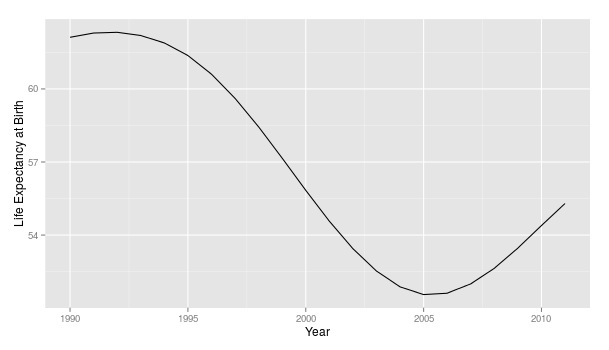
\includegraphics[scale=0.5]{lifeExp.png}
\end{figure}

Around the year 2005 the life expectancy at birth was slighly above 50 years.
Since pension eligibility age is 60 years (and 65 for men until 2009),
there is an almost ten year gap between average life expectancy and pension eligibility.
This gap causes a delayed in the effect of the drop in life expectancy.
The attribition effect of a person passing away at the age of fifty, on the pension recipient base,
will thus only be observed ten years after death.

After the year 2005, life expectancy started rising slowly,
however, as explained above, it will take some time for this effect to disseminate into the pension base.

% Include graph

% stats of people over 65.


\begin{table}[ht!]
\centering
\caption{Children in Households with and without Male Pension Recipients}
\label{sa:ta:hmr}
    \begin{tabular}{l|rrrr}
    \hline
    Year              & 2008   & 2012   & 2013   & Overall \\
    \hline
    Male Recipient    & 612    & 595    & 623    & 1830    \\
    No Male Recipient & 6121   & 6138   & 6110   & 18369   \\
    Ratio of Male Recipients & 0.0909 & 0.0884 & 0.0925 & 0.0906  \\
    \end{tabular}
\end{table}

\begin{table}[ht!]
\centering
\caption{Children in Households with and without Female Pension Recipients}
\label{sa:ta:hfr}
    \begin{tabular}{l|rrrr}
    \hline
    Year                & 2008   & 2012   & 2013   & Overall \\
    \hline
    Female Recipient    & 1637   & 1498   & 1509   & 4644    \\
    No Female Recipient & 5096   & 5235   & 5224   & 15555   \\
    Ratio               & 0.2431 & 0.2225 & 0.2241 & 0.2299  \\
    \end{tabular}
\end{table}


\section{Conclusions and Limitations}
We find two results from out estimations.
Firstly, we find that there is a significant and consistant negative effect of the policy variable \textbf{elig.men.60} on the age-based z-scores
(i.e.~Height for Age and Weight for Height).
Secondly, we find a consistent and negative effect of the men's pension variable (\textbf{w\_spen\_m}) on the Body-Mass-Index Z-scores.
Both of these effect are consistent across the different specifications used in our estimations.

The main impetus for this paper lies in the optimal design of cash transfer schemes,
such as Conditional Cash Transfers (CCTs) and the newly fashionable Uncondional Cash Transfers (UCTs).
Which is the optimal manner in which these grants are distributed, measured along the bars of health,
as well as education and work force participation.
In this paper \parencite[like in][]{duflo2000child,duflo2003grandmothers} we try to address of the issue of differential effects relating to the gender of the cash recipient.

We do this by evaluating the z-scores of anthropometrics of children between the ages of six and sixty months old, living in the same household as recipients of the South-African old-age state pension system. We then compare the z-scores for children living with male pension recipients, which the z-scores of children living with female pension recipients.

This approach is identical to \textcite{duflo2000child,duflo2003grandmothers}, however this analysis offers some additional value.
Firstly, we analyse data around a policy change, which lowers the pension eligibility age for men from 65 to 60,
which brings it at par with women's pension eligibility age.
There are two impeti for further analysis of this data.

Firstly, this partly overcomes major issues with attrition and the associated selection bias.
Since average life expectancy is well below pension eligibility age,
there is a strong indication that such a selection bias issue would be present.
It is also very likely that confounding variables would be effecting both the selection bias, as well as the dependent variable.
With the differential in pension eligibility age, this would make the effect incomparable,
however, as the men's eligibility age is brought to the same as women's, this makes comparison less problematic.
Considering the fact that selection bias in our analysis is comparable, but nevertheless still present,
we note that we cannot automatically draw inferences about the external validity of the results presented here.

Secondly, analysing data around the policy change allows us to employ a Difference-in-Differences estimation (DiD).
Which enables us to draw a causal inference from the treatment effect,
which is ontologically more interesting than a correlation.

We use the South-African National Income Dynamics Survey data
\parencite[in collaboration with The World Bank]{saldru2008nids,saldru2012nids,saldru2013nids}.
This full-panel dataset provides observations from 2008, 2012, and 2013.
The treatment, a policy change which lowers the pension eligibility age for men from 65 to 60, takes place around 2009.
Since we have only one time period before the treatment (the year 2008), we cannot establish the common trend.
This common trend is used to validate the common trend assumption, which unpins the Difference-in-Differences method.
As discussed in \autoref{sa:results}, we find that not establishing the trend proves problematic for our analysis.
Between the years 2008 and 2012,
we see a substantial drop in the number of children living in the same household as a female pension recipient.
Since female pension recipients are unaffected by the policy change, we have to assume that a further exogenous factor is the cause of this drop.

In our estimations we use the Difference-in-Differences method,
which is operationalised a fixed-effect panel estimation with a time effect.
The construct three Right-Hand Side (RHS) model.
The first model is a fixed-effect estimation without the treatment dummy.
The second model is a fixed-effects estimation with the treatment dummy (\textbf{elig.men.60}).
the third model is a fixed-effects estimation with the treatment dummy,
as well as an interaction term with the male pension recipient dummy (\textbf{w\_spen\_m}).

On the Left-Hand Side (LHS) we use four different anthropometric z-scores,
Height-for-Age (HAZ), Weight-for-Age (WAZ), Weight-for-Height (WHZ), and BMI (BMIZ).
The first two z-scores are age based (ABZ), the latter two height based (since height factors in the BMI equation, HBZ).

Combining the three RHS models with the four LHS z-scores gives us twelve estimation equations.
In the estimation of these twelve equations, we find two effects.

Firstly, we find that in for both the Age-Based Z-scores (ABZs),
the treatment dummy is significant for the models 2 and the models 3
(we do not find this in model 1, since it is not included the model 1 equation).
In all cases, the coefficient for the treatment dummy is negative.
Since both these Age-Based Z-scores (ABZs) reflect long-term or past health issues,
this seems to indicate a negative correlation between the policy change on the long-term anthropometrics.
Since this is the treatment dummy, this would suggest a negative causal effect of male pension receipts on child health.
However, as discussed in \autoref{sa:results},
this is likely to be a consequence of the common trend not having been established.
Since we also observe a sharp drop in the number of children living with female pension recipients,
despite the fact that the female pension recipient base in unaffected by the policy change.

Secondly, we find that living with male pension recipient (\textbf{w\_spen\_m}),
is negatively correlated with a the BMI z-scores (\textbf{BMIZ}).
As discussed in \autoref{sa:results}, the Body-Mass-Index Z-score is a convex mapping of the Weight-for-Height z-score.
This can explain the fact that these essentially similar estimations, give different significance levels.
Considering that the use of the Body Mass Index is far more wide spread than the Weight for Height metric,
we believe that the significance of these coefficients carries more weight.
The fact that these coefficients are negative, indicates that for this short-term z-score,
the preferred recipient would be female household members.

In conclusion, we find a negative correlation between the treatment dummy and the long-term ABZs.
This is likely to be a consequence of the common trend not having been established,
since there is also a drop in the number of children living with female pension recipients, which serves as the control group.
Furthermore, we find a negative correlation between the male pension recipient variable (\textbf{w\_spen\_m}) and the short-run \textbf{BMIZ}.

The later result seems to indicate that, at least in the short-run,
the preferred recipient of cash transfers would be a female household member.
As discussed, the selection bias issue in age,
leads to the need for a careful interpretation of the possible external validity of this results.

Regarding the former result, the significant negative coefficient of the treatment variable,
the analysis in \autoref{sa:results} seems to indicate a need to establish the common trend,
at least over the period 2008-2012.
Since the female recipient base in this period serves as a control group, we possibly could establish this, using the evolution here.
Alternatively, it would be possible to establish a trend using statistics on nationwide pension recipients.

\printbibliography
\end{refsection}
